This section describes the hardware components, architecture, and configuration of the mobile robot system used for yaw control and line following.

The hardware components are the same described in Section~\ref{sec:system_configuration}.

The control structure of the system, used for the implementation of the yaw controller, is divided into two layers:
\begin{itemize}
    \item Low-level layer: responsible for maintaining the desired velocities of the left and right wheels using PI controllers.
    \item High-level layer: computes the yaw error from the sensor data and applies a proportional correction to the wheel speed reference, effectively steering the robot back onto the path.
\end{itemize} 

When the robot deviates from the center of the line, the yaw error increases. 
The proportional yaw controller reacts by adjusting the difference between the left and right wheel speeds, thereby rotating the robot toward the line. 
This hierarchical control scheme ensures smooth and responsive tracking of the line.

For the design of the yaw controller, we considered as input the yaw error ($\psi_{err}$) and the output was the control signal for the robot's wheels, i.e. the yaw rate ($\dot{\psi}$), as shown in Figure~\ref{fig:yaw_controller}.
\begin{figure}[H]
    \centering
    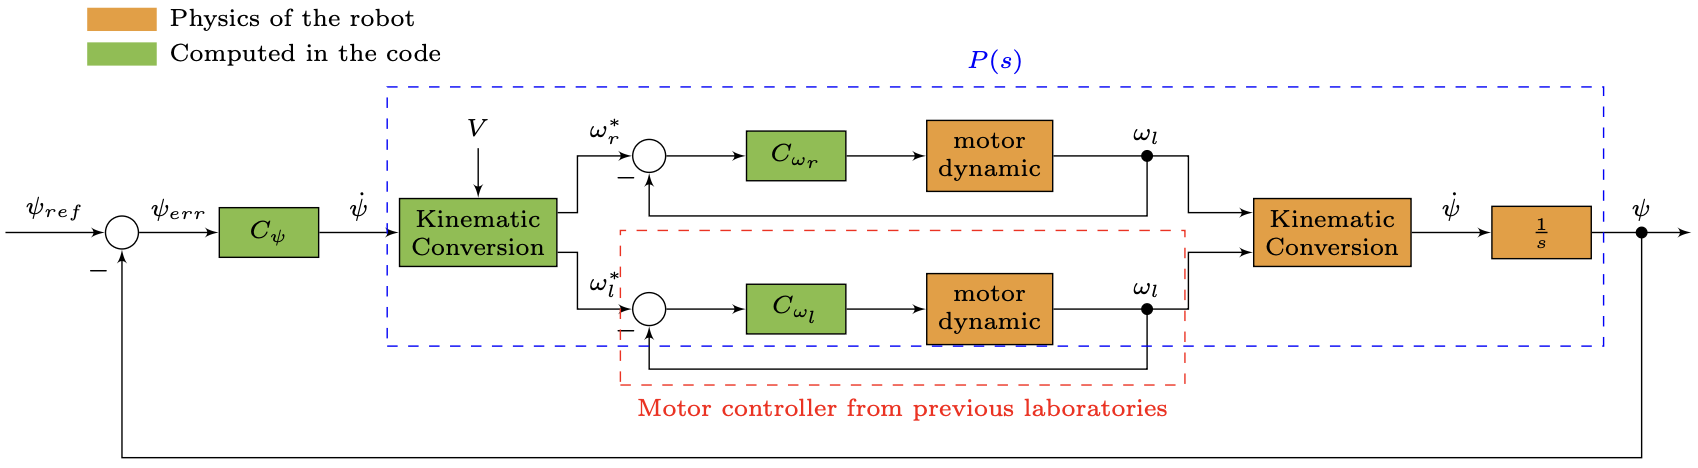
\includegraphics[width=0.7\textwidth]{lab4/figures/yaw_controller.png}
    \caption{Yaw controller}
    \label{fig:yaw_controller}
\end{figure}
